\documentclass[professionalfonts,compress,unicode]{beamer}

\usepackage{amsmath,amssymb}
\usepackage[utf8]{inputenc}
\usepackage{epstopdf}

\usepackage[russian]{babel}

\usepackage{ifthen}

\def\[#1\]{\begin{align*}#1\end{align*}}

\newcommand\myframe[3][dup]{
\ifthenelse{\equal{#1}{}}{}{\ifthenelse{\equal{#1}{dup}}{\subsection{#2}}{\subsection{#1}}}
\frame{\frametitle{#2}{#3}}%
}


\usetheme{Warsaw}
\usecolortheme{uranix}

\setbeamertemplate{headline}
{%
  \begin{beamercolorbox}[sep=0.3cm,wd=\paperwidth]{section in head/foot}%
    \usebeamerfont{frametitle}%
    \vbox{}\vskip-1ex%
    \strut\insertsectionhead\strut\par%
    \vskip-1ex%
  \end{beamercolorbox}%
}
\setbeamertemplate{navigation symbols}{}
\setbeamertemplate{footline}{}
\setbeamertemplate{caption}[numbered]

\renewcommand{\thefootnote}{\fnsymbol{footnote}}

\graphicspath{{images//}}

\title[Нелинейные уравнения]{Задача Коши. Методы Рунге-Кутты. Жесткие задачи}
\author[Цыбулин И.В.]{Скалько Юрий Иванович\\
\textbf{Цыбулин Иван}
\\Шевченко Александр}
\date{}
%\vspace{0.3cm}

\begin{document}

{
\setbeamertemplate{headline}[default]
\frame{
\titlepage
}

%\frame{
%\frametitle{Содержание}
%\small
%%\tiny
%\tableofcontents
%}
}

\section{ }

%\myframe{Материалы по курсу вычислительной математики}
%{
%\begin{itemize}
	%\item 
		%Материалы курса (методички, лекции, учебники и др.) можно найти 
		%на сайте кафедры вычислительной математики
		%{\color{blue} http://crec.mipt.ru/study/materials/compmath/}
	%\item 
		%Любые вопросы по курсу (и не только) можно присылать на почтовый ящик
		%{\color{blue} tsybulinhome@gmail.com}
%\end{itemize}
%}

\def\L{\mathcal{L}}

\section{Обыкновенные дифференциальные уравнения}
\myframe{Задача Коши}
{
	Дано обыкновенное дифференциальное уравнение 1го порядка и начальное условие
	\begin{align*}
	\frac{dy(t)}{dt} &= G(t, y(t))\\
	y(0) &= y_0
	\end{align*}
	Требуется найти решение $y(t)$ при $t \in [0, T]$
}

\section{Методы Рунге-Кутты}
\myframe{Методы Рунге-Кутты}
{
	Методы Рунге-Кутты относятся к \emph{одношаговым методам}, то есть они позволяют по 
	значению решения $u_{n}$ вычислить значение в следующей точке $u_{n+1}$.
	
	Каждый шаг метода состоит из нескольких \emph{стадий}, на которых вычисляются вспомогательные
	наклоны $k$. Вычисление наклонов в специально подобранных промежуточных точках позволяет 
	получить метод с высоким порядком аппроксимации.
}

\myframe[]{Методы Рунге-Кутты}
{
	Каждый метод Рунге-Кутты характеризуется набором коэффициентов $a_{ij}, b_j, c_i$. 
	Один шаг метода проводится по следующей схеме:
	\begin{columns}[T]
	\begin{column}{.5\textwidth}
	\[
	k_1 = G(t_n + c_1 \tau&, u_n + \tau\sum_{j=1}^s a_{1j} k_j)\\
	&\vdots\\
	k_s = G(t_n + c_s \tau&, u_n + \tau\sum_{j=1}^s a_{sj} k_j)\\
	\frac{u_{n+1} - u_n}{\tau} &= \sum_{j=1}^s b_j k_j
	\]
	\end{column}
	\begin{column}{.5\textwidth}
	\begin{figure}%
	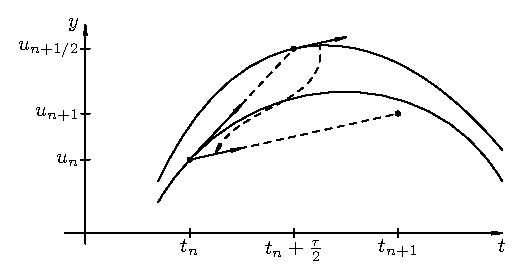
\includegraphics[width=\columnwidth]{rk-0.eps}%
	\[
	k_1 &= G(t_n, u_n)\\
	k_2 &= G\left(t_n + \frac{\tau}{2}, u_n + \frac{\tau}{2} k_1\right)\\
	&\frac{u_{n+1} - u_n}{\tau} = k_2
	\]	
	\end{figure}
	\end{column}
	\end{columns}
}
\myframe{Таблица Бутчера}
{
	Коэффициенты $a_{ij}, b_j, c_i$ удобно представлять в виде \emph{таблицы Бутчера}
	\begin{equation*}
	\begin{array}{c|cccccc}
	c_1 & a_{11} & a_{12} & \dots & a_{1s}\\
	c_2 & a_{21} & a_{22} & \dots & a_{2s}\\
	\vdots & & & \ddots & \\
	c_s & a_{s1} & a_{s2} & \dots & a_{ss}\\
	\hline
	& b_1 & b_2 & \dots & b_s
	\end{array}
	\end{equation*}
	Например, явному методу средней точки соответствует таблица
	\begin{equation*}
	\begin{array}{c|cccccc}
	0 & 0 & 0\\
	\frac{1}{2} & \frac{1}{2} & 0\\
	\hline
	& 0 & 1
	\end{array}
	\end{equation*}
}

\myframe{Явные, полуявные и неявные методы Рунге-Кутты}
{
	В зависимости от коэффициентов $a_{ij}$ вычисления наклонов $k_i$ могут 
	происходить по-разному. 
	
	Если матрица $a_{ij}$ имеет ненулевые элементы ниже главной диагонали ($a_{ij} = 0, i\geq j$),
	то метод называется \emph{явным}. При этом все наклоны $k_i$ вычисляются через предыдущие без необходимости
	решать уравнения.
	
	Если матрица $a_{ij}$ имеет ненулевые элементы и на главной диагонали ($a_{ij} = 0, i > j$),
	то метод называется \emph{полуявным}. При этом все наклоны $k_i$ вычисляются последовательно из уравнений.

	Иначе, метод называется \emph{неявным}, и необходимо решать систему уравнений для всех $k_i$ одновременно.
}

\myframe{Аппроксимация}{
	Поскольку метод Рунге-Кутты определяется своими коэффициентами, можно сформулировать условия на коэффициенты метода, при котором 
	он имеет определенный порядок аппроксимации. Найдем условия первого и второго порядков, для этого подставим $u_n = [y]_n$, где $y(t)$ --- 
	решение задачи Коши:
	\[
	k_i &= G(t_n + c_i \tau, [y]_n + \tau \sum\nolimits_{j=1}^s a_{ij} k_j) =\\
			&= [G]_n + \tau c_i [G_t]_n + \tau \sum\nolimits_{j=1}^s a_{ij} [G_y]_n k_j + O(\tau^2) = \\
			&= [G]_n + \tau c_i [G_t]_n + \tau \sum\nolimits_{j=1}^s a_{ij} [G_y]_n \Big([G]_n + O(\tau)\Big) + O(\tau^2) = \\
			&= [G]_n + \tau c_i [G_t]_n + \tau \sum\nolimits_{j=1}^s a_{ij} [G_y]_n [G]_n + O(\tau^2)
	\]
}

\myframe[]{Аппроксимация} {
	\[
	k_i &= [G]_n + \tau c_i [G_t]_n + \tau \sum_{j=1}^s a_{ij} [G_y]_n [G]_n + O(\tau^2)\\
	\sum_{j=1}^s b_j k_j &= 
	\sum_{j=1}^s b_j [G]_n + \tau \sum_{j=1}^s b_j c_j [G_t]_n + \tau \sum_{i,j=1}^s b_i a_{ij} [G_y]_n[G]_n \\
	\frac{[y]_{n+1}-[y]_n}{\tau} &= [G]_n + \frac{\tau}{2}[G_t]_n + \frac{\tau}{2}[G_y]_n [G]_n + O(\tau^2)
	\]
	\pause
	Условие $1$-го порядка аппроксимации: $\displaystyle \sum_{j=1}^s b_j = 1$.
	
	Условия $2$-го порядка аппроксимации: $\displaystyle \sum_{j=1}^s b_j c_j = \sum_{i,j=1}^s b_i a_{ij} = \frac{1}{2}$.
}

\myframe[]{Аппроксимация} {
	Бутчер доказал несколько теорем о связи порядка аппроксимации и количества стадий у методов Рунге-Кутты. 
	Явные методы с $s<5$ стадиями могут иметь порядок не выше $s$, но после $s=5$ стадий наступает, так называемый,
	\emph{первый барьер Бутчера}, и порядок аппроксимации не превышает $s-1$. При увеличении $s$ возникают все новые барьеры, понижающие 
	порядок аппроксимации.
	
	Однако, для неявных методов ограничение не такое строгое. Например есть семейство методов (Гаусса), у которых порядок аппроксимации $2s$ при любом числе стадий.
}

\myframe{Устойчивость} {
	Если правая часть ОДУ $G(t,y)$ липшицева по $y$ с константой $L$
	$$|G(t,y) - G(t,v)| \leq L ||y-v||,$$
	то несложно показать, что константа устойчивости для методов Рунге-Кутты порядка
	$C \sim \exp\{O(L)T\}$. Следовательно, имеет место сходимость решения разностной задачи к решению дифференциальной задачи.

	Но в случаях, когда $LT \gg 1$ константа устойчивости становится огромной.
	Вспоминая, что ошибка сходимости связана с ошибкой аппроксимации
	$$\varepsilon_\text{сх} = C	\varepsilon_\text{аппр}(\tau),$$
	единственный способом получить приемлимую точность --- сделать ошибку
	аппроксимации очень маленькой, то есть сильно уменьшить $\tau$.
}

\section{Жесткие задачи Коши}
\myframe{Жесткие задачи} 
{
	Жесткие системы ОДУ описывают, как правило, одновременно проходящие очень быстрые и очень медленные процессы. 
	Например, в задачах химической кинетики бывают различия в скоростях реакций до $10^{15}$ раз.
	\pause
	Оказывается, что быстро протекающие процессы, даже быстро закончившись, продолжают влиять на численное решение задачи, 
	вынуждая рассчитывать решение с очень малым шагом по времени, где это, казалось бы, совершенно не требуется (решение довольно гладкое).
}

\myframe{Поле решений жесткой задачи} {
	\begin{columns}[T]
	\begin{column}{.4\textwidth}
	\vspace{1in}
	Поле решений уравнения
	\[
	y' = -50(y+\cos x)
	\]
	\vspace{1in}
	\end{column}
	\begin{column}{.6\textwidth}
	\begin{figure}%
	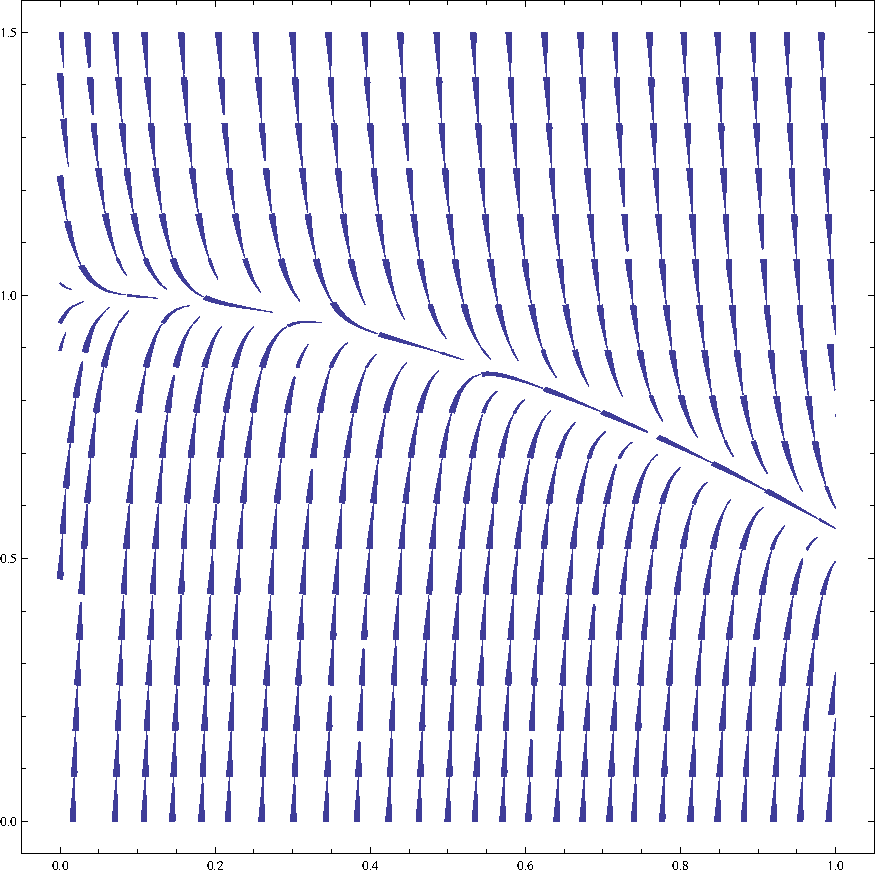
\includegraphics[width=\columnwidth]{stiff.pdf}%
	\end{figure}
	\end{column}	
	\end{columns}
}

\myframe{Численное решение жесткой задачи} {
	\begin{columns}[T]
	\begin{column}{.4\textwidth}
	\vspace{.4in}
	
	Явный метод Эйлера при $\tau=0.04$
	\[
	\frac{u_{n+1}-u_n}{\tau} = -50(u_n+\cos t_n)
	\]
	\vspace{.4in}
	
	Неявный метод Эйлера при $\tau=0.1$
	\[
	\frac{u_{n+1}-u_n}{\tau} = -50(u_{n+1}+\cos t_{n+1})
	\]
	
	\vspace{.4in}
	\end{column}
	\begin{column}{.6\textwidth}
	\begin{figure}%
	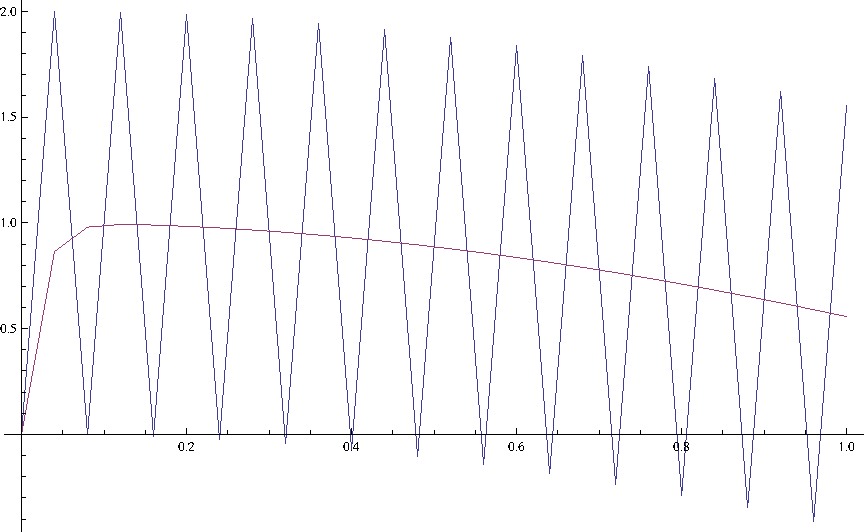
\includegraphics[width=.8\columnwidth]{euler.pdf}%
	
	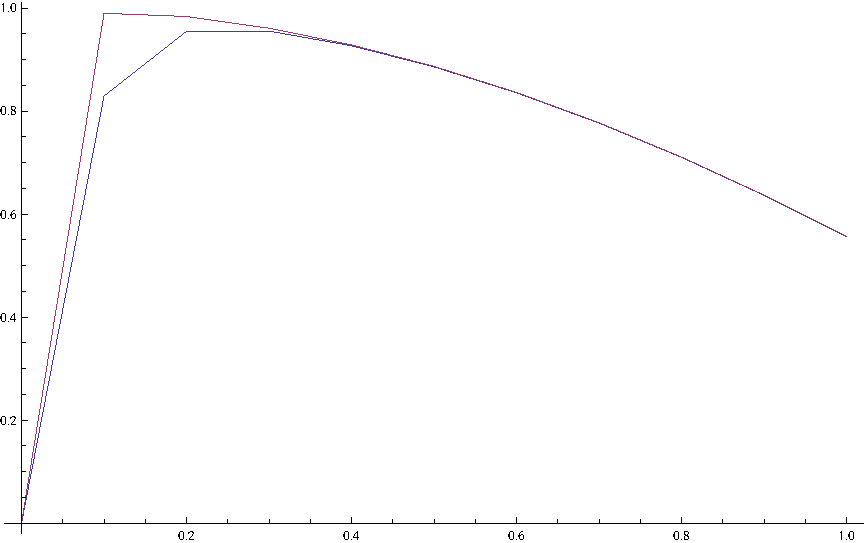
\includegraphics[width=.8\columnwidth]{euleri.pdf}%
	\end{figure}
	\end{column}	
	\end{columns}
}

\myframe{Жесткая задача}{
	Можно дать следующее определение:
	
	Жесткая задача --- это такая задача, у которой собственные числа матрицы Якоби $G_y$ 
	разбиваются на две части --- мягкую часть спектра $|\lambda_i| < \ell$ и жесткую часть спектра $\operatorname{Re} \Lambda_i < -L$, причем $\ell \ll L$
	\begin{figure}%
	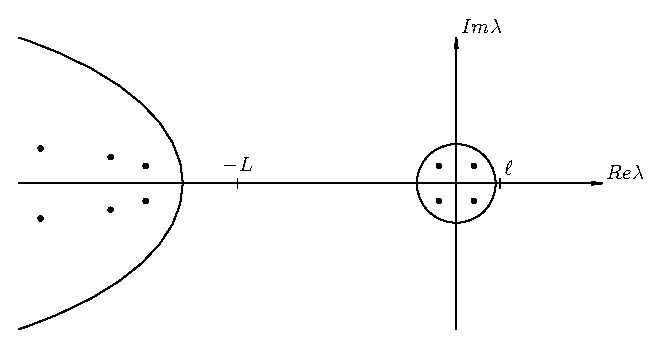
\includegraphics[width=\columnwidth]{sp.eps}%
	\caption{}%
	\label{}%
	\end{figure}
}

\myframe{Функция устойчивости}{
	Выяснить, как на жестких задачах себя ведет тот или иной метод, можно на модельном уравнении
	\[
	y' = \lambda y,\quad \operatorname{Re} \lambda < 0
	\]
	Все линейные численные методы для решения этого уравнения будут иметь вид
	\[
	u_{n+1} = r(\lambda \tau) u_n,
	\]
	где $r(z)$ --- функция, зависящая только от метода. Эта функция называется \emph{функцией устойчивости метода}
	Если при данном сочетании $\lambda$ и $\tau$ значение функции $r(\lambda \tau)$ по модулю больше единицы, решение будет экспоненциально возрастать, что
	противоречит реальному поведению решения при $\operatorname{Re} \lambda < 0$.
	Область комплексной плоскости $\mathbb{C}$, в которой $|r(z)| < 1$ называется \emph{областью устойчивости метода}
}

\myframe[]{Функция и область устойчивости}{
	Если при данном $\tau$ вся жесткая часть спектра попадает в область устойчивости, она гарантированно не будет экспоненциально возрастать, и 
	решать систему ОДУ можно только обращая внимание на мягкую часть спектра. 
	
	Для явного метода Эйлера функция устойчивости
	\begin{columns}[T]
	\begin{column}{.5\textwidth}	
	\[
	u_{n+1} &= (1 + \tau \lambda)u_n = (1+z) u_n\\
	r(z) &= 1+z
	\]
	\end{column}
	\begin{column}{.5\textwidth}	
	\begin{figure}%
	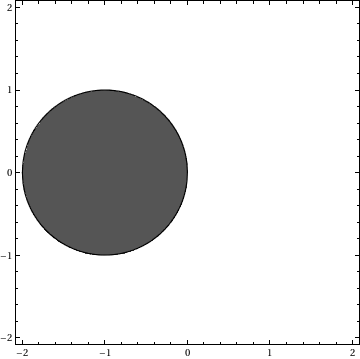
\includegraphics[width=.8\columnwidth]{euler.png}%
	\end{figure}
	\end{column}	
	\end{columns}
}

\myframe[]{Функция и область устойчивости}{
	Для неявного метода Эйлера функция устойчивости
	\begin{columns}[T]
	\begin{column}{.5\textwidth}	
	\[
	u_{n+1} &= \frac{u_n}{1 - \tau \lambda} = \frac{u_n}{1 - z}\\
	r(z) &= \frac{1}{1-z}
	\]
	\end{column}
	\begin{column}{.5\textwidth}	
	\begin{figure}%
	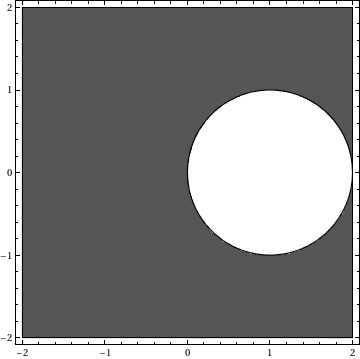
\includegraphics[width=.8\columnwidth]{euleri.png}%
	\end{figure}
	\end{column}	
	\end{columns}
}

\myframe[A- и L- устойчивость]{$A$- и $L$-устойчивость} {
	По виду области устойчивости методы можно дополнительно классифицировать. Это позволяет выбирать метод,
	наиболее подходящий для конкретного вида жесткой части спектра задачи.
	
	\begin{itemize}
		\item $A$-устойчивость означает, что во всей полуплоскости $\operatorname{Re} z < 0$ метод устойчив, т.е. $|r(z)| < 1$.
		\item $A(\alpha)$-устойчивость означает, что в конусе $|\operatorname{Im} z| < -\tg \alpha \operatorname{Re} z$ метод устойчив. $A$-устойчивость 
		эквивалентна $A(90^\circ)$
		\item $L$-устойчивость означает, что $\lim_{z \rightarrow -\infty} r(z) = 0$. Это свойство говорит, что при большом шаге $\tau$ жесткая часть спектра 
		стремится к нулю достаточно быстро.
	\end{itemize}
}

\myframe{Функция устойчивости методов Рунге-Кутты} {
	Для методов Рунге-Кутты функцию устойчивости можно вычислить по формуле
	\[
	r(z) = \frac{\det(E - zA + zeb^T)}{\det(E - zA)}, 
	\]
	где $e$ --- единичный вектор.
	\pause	
	Для случая явного метода, $r(z)$ является многочленом от $z$ степени $s$ (число стадий).
	Но также, $r(z)$ должен с точностью до $O(z^{p+1})$ совпадать с разложением $e^z$ в ряд по $z$ (аппроксимация порядка $p$).
	Если $s = p$, то $r(z)$ есть просто первые $s+1$ членов ряда Тейлора функции $e^z$.
}

\myframe{Области устойчивости методов Рунге-Кутты 1-4 порядка}{
\begin{figure}%
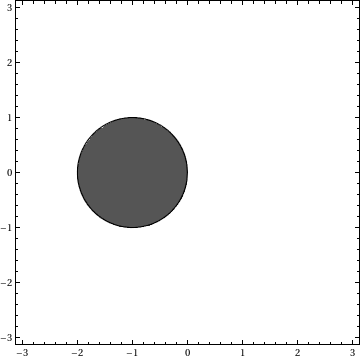
\includegraphics[height=.4\textheight]{rk1.png}%
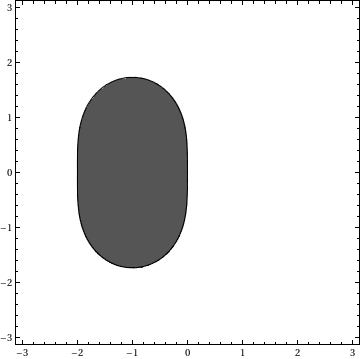
\includegraphics[height=.4\textheight]{rk2.png}%

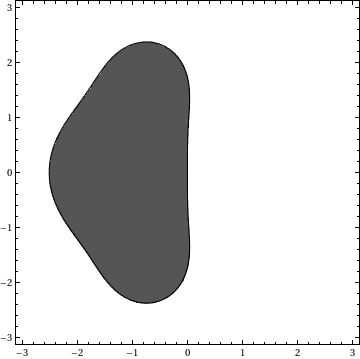
\includegraphics[height=.4\textheight]{rk3.png}%
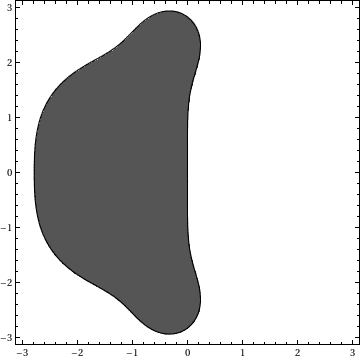
\includegraphics[height=.4\textheight]{rk4.png}%
\end{figure}
}
%%%%%%%%%%%%%%%%%%%%%%%%%%%%%%%%%%%%%%%%%%%%%%%
%%%%%%%%%%%%%%%%%%%%%%%%%%%%%%%%%%%%%%%%%%%%%%%
%%%%%%%%%                            %%%%%%%%%%
%%%%%%%%%%%%%%%%%%%%%%%%%%%%%%%%%%%%%%%%%%%%%%%
%%%%%%%%%%%%%%%%%%%%%%%%%%%%%%%%%%%%%%%%%%%%%%%
{
\setbeamertemplate{headline}[default] 
\frame{
	\begin{center}
	{\Huge Спасибо за внимание!}
	\end{center}
	\bigskip
	\begin{center}
	{\color{blue}{tsybulin@crec.mipt.com}}
	\end{center}
	}
}

\end{document}
